\documentclass[border=3mm,tikz]{standalone}

\usetikzlibrary{arrows,positioning}

    \begin{document}
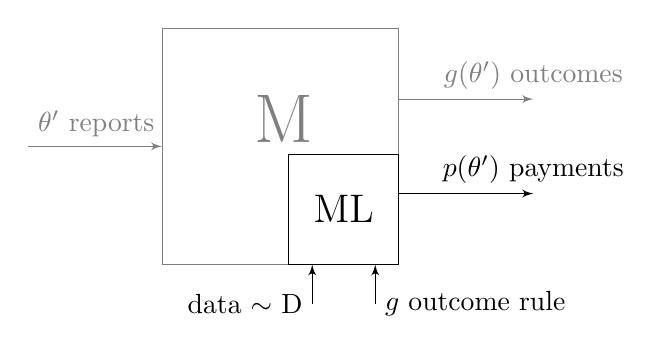
\begin{tikzpicture}[
node distance = 6mm and 17mm
]
\node (m) [gray, draw,minimum size=30mm, label={[label distance=-2cm, gray]10:\Huge{M}}] {};
\node (n) [draw,minimum size=14mm] at (0.8,-0.8) {\Large{ML}};

%
\coordinate[left = of m.west]   		(a1);
\coordinate[above right= of m.east]  	(b1);
\coordinate[below right= of m.east]  	(b2);


\coordinate(svm1) at (0.4,-2);
\coordinate(svm2) at (0.4,-1.5);
\coordinate(svm3) at (1.2,-2);
\coordinate(svm4) at (1.2,-1.5);


\draw[-latex', gray]  (a1) node[above right] {$\theta'$ reports} -- (a1-| m.west);
\draw[-latex', gray] (m.east |- b1) -- (b1) node[above] {$g(\theta')$ outcomes};
\draw[-latex'] (m.east |- b2) -- (b2) node[above] {$p(\theta')$ payments};


\draw[-latex']  (svm1) node[left] {data $\sim$ D} -- (svm1 |- svm2);
\draw[-latex']  (svm3) node[right] {$g$ outcome rule} -- (svm3 |- svm4);

\end{tikzpicture}    	
    \end{document}